\chapter{Model Application}
\label{chp:chapter4}
\graphicspath{{figures/}{figures/chapter4/}}

\section{Overview}
In this chapter, model described in Chapter 3 is applied to evaluate the relative systemic
criticality of highway links on a statewide network using a logit-based model
sensitive to changes in route path, destination choice, and mode choice. To do this, the model is applied to scenarios
where critical highway links have been removed from the USTM network. This
chapter includes first, a detailed analysis of a single scenario, where I-80
between Salt Lake and Tooele Counties is severed. Then, the model
output is compared to an alternative method that measures only the change in travel
time and does not allow for mode or destination choice. The model was then
applied to 41 individual scenarios, with 40 of those scenarios involving link
closure scenarios throughout the state.

\section{Vulnerable Link Identification}
In order to determine which links on the USTM network might be most critical,
a method must be developed to identify links of interest for analysis. Currently, UDOT uses
an online Risk Priority Analysis GIS toolkit created by both BIO-WEST and UDOT,
which grades highway links based on several criteria, including:
\begin{itemize}
   \item {Threat (e.g., rock fall/flood, etc.)}
   \item {Probability of threat}
   \item {Cost to replace}
   \item {User Costs (e.g., AADT and Truck Volume)}
\end{itemize}
This tool, combined with information gathered from the research team and UDOT
officials, 40 locations of interest were identified for analysis. Each link was
identified due to its location in relation to
population centers, remote geographic location, and proximity to other highway
facilities, or because the link was known to be at risk due to geologic or geographic features, or
because it was a suspected choke point in the network.

After identifying locations of interest on the network, the model is applied to
each of the selected scenarios. In each scenario, an individual highway
link is removed from the model highway network. Some of the links identified
by \citeauthor{aem2017}, the \citeauthor{riskanalysis}, or the research team are
also examined. The locations of each of the 40
selected links are shown in Figure \ref{fig:linksmap}, and are then analyzed one by one. The
final results of each scenario are presented in the following sections. First, a detailed analysis of a single
scenario are presented, however.

\section{Analysis of I-80 at Tooele / Salt Lake County Line}

This section outlines an in-depth analysis that was conducted to ensure
the presented model was accurately describing trips likely behavior with OD pairs in the
targeted area around a severed link. This analysis was done on a link between
Tooele and Salt Lake City, Utah, which is located close to the county line. A map, with the approximate
location of road closure can be seen in Figure \ref{fig:tooelemapwithcone}.

\begin{figure}

{\centering 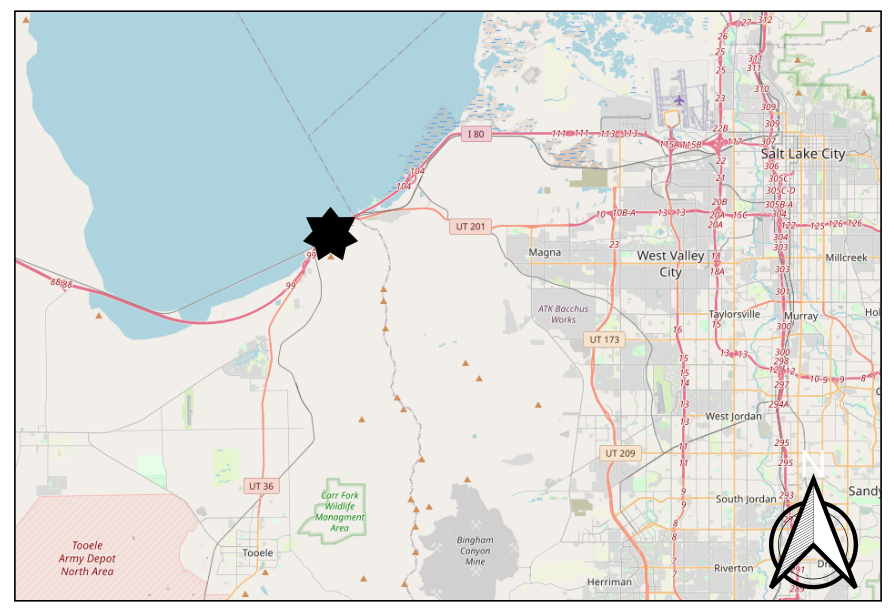
\includegraphics[width=0.75\linewidth]{figures/chapter4/tooelemapwithcone.png}

}

\caption{Approximate location of the I-80 closure on the Tooele/SL County line.}\label{fig:tooelemapwithcone}
\end{figure}

This detailed analysis is useful because it
provides a closer look at the way the model works, capturing trips
between two population centers. Scenario 50, which is located along I-80 between Tooele and Salt Lake Counties
was examined here. The localized analysis shows that the majority of trips
affected by damage to this link either originate or terminate in one of the
two counties, as expected. These results can be seen in Table
\ref{tab:tooeletable}. Another method used to compare results is
the travel time method,
which serves to capture trips that have fixed OD pairs such as freight and
recreational trips. This localized analysis also looks at this method.

Table \ref{tab:tooeletable} compares the overall cost estimates between the
logsum and travel time methods, and the specific cost for trips originating in
Tooele County. We can see that the logsum
method captures \$123,042.44 of expenses experienced by road users due to the closure of the
link across the whole network. Specifically, for trips originating in Tooele County, the logsum analysis using the Resiliency
Model captures \$118,766.19 of
expense, which is approximately 96.52\% of the total expense experienced
statewide. A further breakdown of expenses experienced at the local level
for trips originating in Tooele County
can be seen Table \ref{tab:tooeletable}.

The data supports the conclusion that the model is effectively
capturing trips originating in Tooele based on the amount of cost captured,
shown in Table \ref{tab:tooeletable2} as a percent capture rate. Additionally, when the
travel time method of analysis is examined, it can be seen that the cost estimated
is equatl to \$11,377,504.92 for the whole network, and \$781,015.04 for only
those trips originating in Tooele County. These two estimates include Freight
trips, which have much higher cost estimates than do any of the other trip purposes.
Though some Freight trips do originate in Tooele County, many more Freight trips traverse
I-80, which cause the cost estimate to increase greatly when the travel time method
is used.

In order to better visualize the change in DCLS experienced in Toole and Salt Lake
Counties, several choropleth maps were generated. Each of the three maps depicts
the change in DCLS using a different method of analysis. First, the total change in DCLS is calculated using,
\begin{equation}
  DCLS_{{HBW}_{Original}} - DCLS_{{HBW}_{Broken}}
\end{equation}
is shown in Figure \ref{fig:totchangemap}.
Second, the percent change in DCLS is calculated using,
\begin{equation}
  \frac{DCLS_{{HBW}_{Original}} - DCLS_{{HBW}_{Broken}}}{{DCLS_{{HBW}_{Original}}}}
\end{equation}
is shown in Figure \ref{fig:percentchangemap}. Finally, The total change in DCLS weighted by the
number of households located within a TAZ is calculated using,
\begin{equation}
  HH * DCLS_{{HBW}_{Original}} - DCLS_{{HBW}_{Broken}}
\end{equation}
is shown in Figure \ref{fig:hhmap}. In each of these choropleths,
darker red zones represent zones with greater change when compared with lighter zones.
\begin{figure}[H]
\begin{center}
{\centering 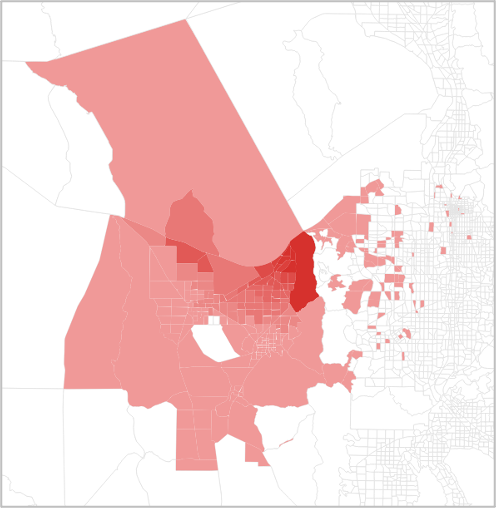
\includegraphics[width=0.50\linewidth]{figures/chapter4/totalchangechoropleth.png}}

\caption{Total change in DCLS by TAZ in Tooele and Salt Lake Counties.}
\label{fig:totchangemap}
\end{center}
\end{figure}

\begin{figure}[H]
\begin{center}
{\centering 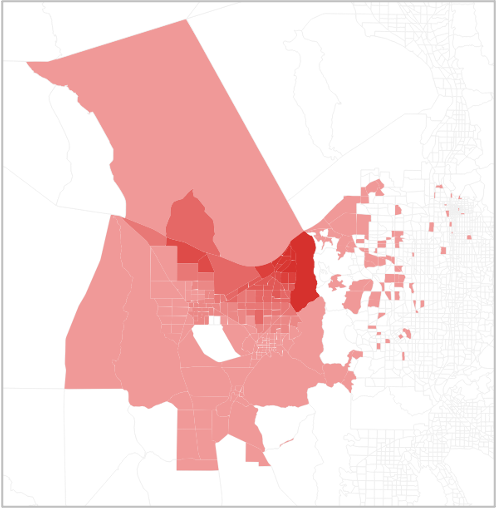
\includegraphics[width=0.50\linewidth]{figures/chapter4/percentchangechoropleth.png}}

\caption{Percent change in DCLS by TAZ in Tooele and Salt Lake Counties.}
\label{fig:percentchangemap}
\end{center}
\end{figure}

\begin{figure}[H]
  \squeezeup
\begin{center}
{\centering 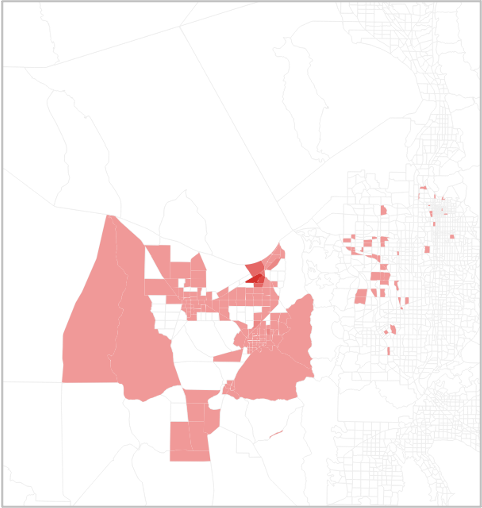
\includegraphics[width=0.50\linewidth]{figures/chapter4/populationweightedchangechoropleth.png}}

\caption{Change in DCLS weighted by households located in a TAZ in Tooele and Salt Lake Counties}
\label{fig:hhmap}
\end{center}
\end{figure}

\squeezeup
\squeezeup
\squeezeup
\squeezeup
\squeezeup
\pagebreak
Overall, two key findings are drawn from this localized analysis of the changes caused by linkn loss at the Tooele/Salt Lake County Line:
\begin{itemize}
  \item {Cost estimates are different by trip purpose and overall depending on
  which estimation method is used}
  \item {The majority of cost for this link is generated by freight trips}
\end{itemize}
The logsum and travel time methods can be broken down into the overall costs and the
comparable costs. The comparable costs are made up of those purposes which are
included in both the presented model and in the travel time method for determining
cost. HBW, HBO, and NHB trip purposes can be compared because all three trip purposes
are represented by each method of cost estimation.

\begin{table}
\caption{\label{tab:tooeletable}Localized Analysis Results}

\centering
%\begin{adjustbox}{width=0.9\textwidth}
\begin{tabular}[t]{lrrrr}
\toprule
Trip Purpose & \multicolumn{2}{c}{ \makecell{Whole Network Cost\\ (Dollars per Day)}} & \multicolumn{2}{c}{\makecell{Tooele Cost \\(Dollars per Day)}}\\
\midrule
 & \makecell{Logsum\\ Method} & \makecell{Travel Time\\ Method} & \makecell{Logsum \\Method} & \makecell{Travel Time\\ Method}\\
\midrule
HBW & \$65,655.13 & \$244,275.72 & \$64,555.39 & \$240,181.80\\
HBO & \$49,851.54 & \$108,412.94 & \$46,793.14 & \$102,699.90\\
NHB & \$7,535.78 & \$84,712.36 & \$7,417.66 & \$77,025.58\\
\midrule
\addlinespace
REC & \$ -  & \$398.72 & \$ -  & \$208.74\\
XXP & \$ -  & \$55,870.17 & \$ - & \$ - \\
Freight & \$ -  & \$10,883,835.01 & \$ -  & \$360,899.92\\
\midrule
HBW, HBO, NHB Total & \$123,042.44 & \$437,401.02 & \$118,776.19 & \$419,907.28\\
Total &  & \$11,377,504.92 &  & \$781,015.04\\
\bottomrule
\end{tabular}
%\end{adjustbox}
\end{table}


\begin{table}

\caption{\label{tab:tooeletable2}Localized Analysis Cost Capture Percentage Rates}
\centering
\begin{tabular}[t]{ccc}
\toprule
 & Logsum & Travel Time\\
\midrule
HBW & 98.32\% & 98.32\% \\
HBO & 93.86\% & 94.73\% \\
NHB & 98.43\% & 90.93\% \\
\bottomrule
\end{tabular}
\end{table}

The travel time method measures the difference in travel time between the base
scenario and any other scenario caused by link closure, and then multiplies that
difference by the VOT for each trip purpose and the number of trips estimated for
each trip purpose. For external trips, freight trips, and REC trips, these were all
extracted directly from USTM. Attempting to include a calculation of the costs
associated with increased travel time for freight trips, external trips, and REC
trips allows a better estimation of the true cost experienced by all road users, not
just those that are included in the model.

The HBW, HBO, and NHB purposes are estimated using the logsum portion of the
model. Calculating the costs associated with the change in logsum
provides estimations of the costs experienced by road users due to link loss
that account for user choice of mode and destination. The logit-based model
employed in the presented model ultimately provides lower estimates of the
total dis-benefit, and therefore cost, experienced by road users due to link
degradation or loss for the purposes included for analysis. However, the
logsum calculation is only used for three purposes in the USTM model. A way to
account for freight trips, REC trips, and trips that occur between external
nodes must also be found. These trip purposes typically have fixed origins
and destinations. As such, a way to account for all purposes must be developed.
Thus, by combining elements from the travel time method and the logsum model,
an estimate can be made that represents all traffic on the USTM network.

\begin{figure}

{\centering 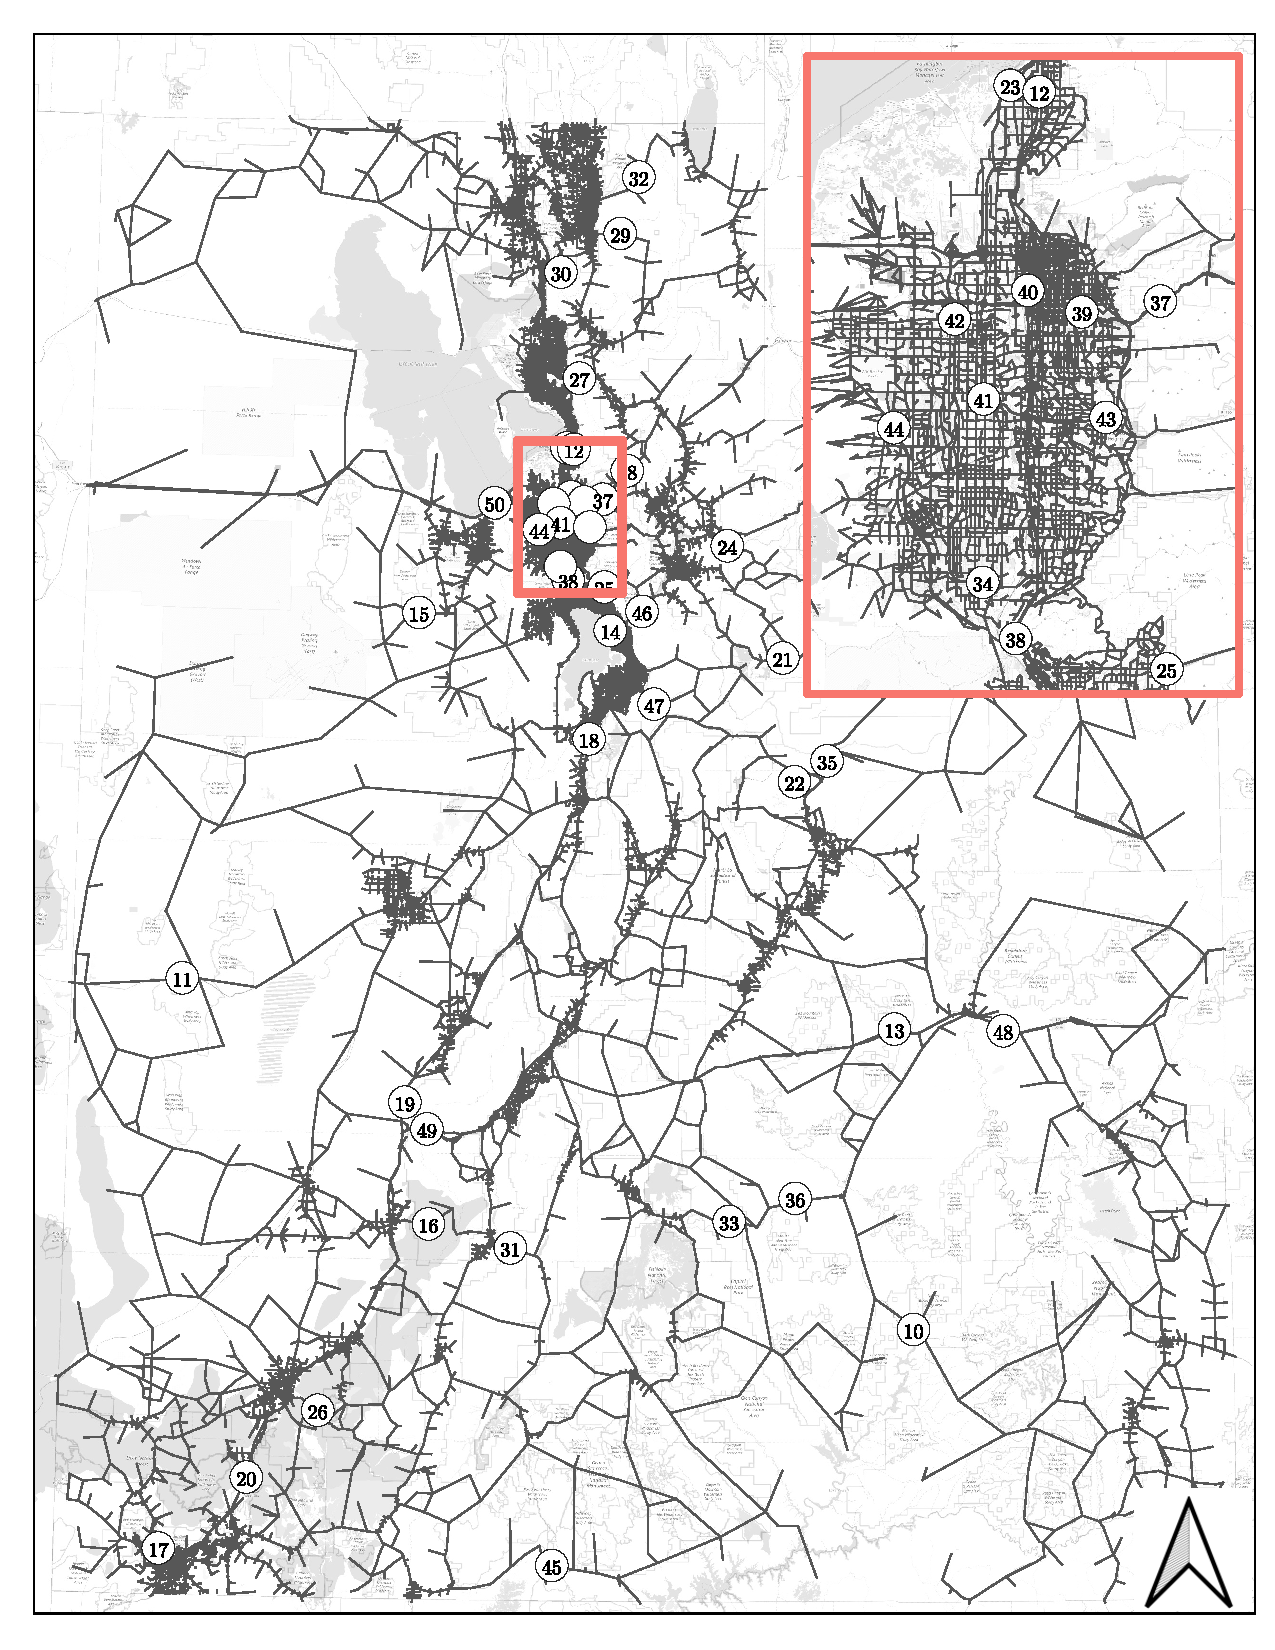
\includegraphics[width=0.95\linewidth]{figures/chapter4/resiliency_links_map.pdf}}

\caption{Links Identified for Analysis.}
\label{fig:linksmap}
\end{figure}

\section{Model Results}

The following section presents the results of the 40 scenarios analyzed.
First, Figure \ref{fig:linksmap} shows the geographic location of each of the
40 links analyzed, where the links are numbered starting with 10. Then,
Table \ref{tab:linkresults} shows each of the scenarios we examined,
labeled simply as ``10'' for Scenario 10, and ``11'' for Scenario 11, along with the
change in accessibility, \(\Delta_{Logsum}\), and the Cost Value in dollars per day
associated with link closure. Other identifying information, such as route
numbers or street names and geographic or other identifying descriptions about
the locations where the link was cut, are also provided.

The logsum method results are shown in Table \ref{tab:linkresults}.
The results are ranked from the road with the largest (most positive
cost) to the road with the smallest cost. We can see that Scenario 27, which
corresponds to I-84 between Ogden and Morgan, experiences the largest cost
per day according to the model. Following Scenario 27, Scenarios 50, 37, 30,
and 17 make up the five most critical roads according to the cost estimation
provided by the model. Each of the roads in these scenarios --- with the exception
of SR-18 in St. George --- is an interstate or state highway facility in
northern Utah, which is heavily populated. Following these five scenarios, are
Scenarios 46, 38, 18, 42, and 41. Each of these facilities are located in northern Utah as well.
Some scenarios, such as Scenario 10,
Scenario 11, or Scenario 33, are roads that are located in remote parts of the state, and
experience no measurable change to HBW, HBO, or NHB traffic. This is
likely due to the remoteness of the geographic location of the highway
link that was cut. Additionally, a few scenarios returned positive benefits, which is not entirely intuitive. These results will be discussed in greater depth later in this chapter. A ranking is provided for all of the scenarios examined
using the logsum method in Table \ref{tab:linkresults}.

\begin{table}
\caption{\label{tab:linkresults}Logsum Analysis Results}
\centering
\begin{tabular}[t]{crrll}
\toprule
Scenario & $\Delta$ Logsum & \makecell{Cost \\(per Day)} & Route & Location\\
\midrule
27 & -23830.208 & \$148,938.80 & I-84 & between Ogden and Morgan\\
50 & -19686.788 & \$123,042.42 & I-80 & between SLC and Tooele\\
37 & -8932.691 & \$55,829.31 & I-80 & in Parley's Canyon\\
30 & -7511.948 & \$46,949.67 & US-91 & between Brigham City \& Mantua\\
17 & -5243.828 & \$32,773.92 & SR-18 & just North of St. George\\
46 & -4911.457 & \$30,696.60 & SR-189 & up Provo Canyon near Vivian Park\\
38 & -4422.194 & \$27,638.71 & I-15 & at the Point of the Mount\\
18 & -3186.967 & \$19,918.54 & I-15 & in Rocky Ridge (between Payson \& Nephi)\\
42 & -2657.614 & \$16,610.08 & Bangerter & near West Valley City\\
41 & -1700.167 & \$10,626.04 & I-215 & near Taylorsville\\
25 & -1139.020 & \$7,118.87 & Timp Hwy & at the mouth of AF Canyon\\
24 & -387.467 & \$2,421.66 & UT-35 & outside of Francis\\
23 & -297.882 & \$1,861.76 & Legacy & near West Bountiful\\
20 & -253.712 & \$1,585.70 & I-15 & near New Harmony\\
47 & -142.671 & \$891.69 & US-6 & Spanish Fork Canyon at Diamond Fork Rd\\
26 & -125.740 & \$785.87 & SR-14 & in Cedar Canyon\\
15 & -67.634 & \$422.71 & SR-199 & near Rush Valley\\
32 & -60.883 & \$380.51 & US-89 & between Logan and Bear Lake\\
14 & -45.386 & \$283.66 & I-15 & in Orem between Univ. Ave \& Center St\\
29 & -41.595 & \$259.96 & SR-101 & East of Hyrum\\
31 & -40.108 & \$250.67 & SR-62 & East of Kingston\\
22 & -30.394 & \$189.96 & US-6 & in Carbon County North of Helper\\
49 & -17.768 & \$111.05 & I-70 & near Richfield \& Fillmore\\
45 & -17.029 & \$106.43 & US-89 & near Arizona Border\\
21 & -11.267 & \$70.41 & US-40 & East of Strawberry Reservoir\\
36 & -10.170 & \$63.56 & SR-24 & near Steamboat Point\\
16 & -9.724 & \$60.77 & SR-153 & between Beaver \& Junction\\
48 & -9.717 & \$60.73 & I-70 & near Green River (NW of Moab)\\
19 & -7.623 & \$47.64 & I-15 & near I-70 \& Fillmore\\
35 & -3.762 & \$23.51 & SR-191 & between Helper \& Duchesne\\
13 & -0.135 & \$8.40 & I-70 & at Dragon Point (W of Green River)\\
28 & -0.103 & \$0.64 & SR-65 & border of Salt Lake \& Morgan Counties\\
10 & 0.000 & \$0.00 & SR-95 & near Hite\\
11 & 0.000 & \$0.00 & US-6 & near King Top\\
33 & 0.000 & \$0.00 & SR-24 & in Capitol Reef National Park\\
12 & 894.999 & -\$5,593.74 & I-15 & in Bountiful\\
44 & 2149.291 & -\$13,433.06 & UT-85 & West of West Jordan\\
43 & 4043.132 & -\$25,269.57 & I-215 & near Cottonwood Heights\\
40 & 5576.276 & -\$34,851.72 & I-15 & in SLC between 2100 S \& 1300 S\\
39 & 7434.744 & -\$46,467.15 & I-80 & in SLC near Sugar House and 1300 E\\
34 & 9362.283 & -\$58,514.26 & Bangerter & near Bluffdale\\
\bottomrule
\end{tabular}
\end{table}


\subsection{Scenario Comparison}
Table \ref{tab:comparison} contains a comparison of the results of the logsum
and travel time methods of cost estimation for all 40 scenarios. In the results,
it can be seen that first 10 scenarios differ from the logsum ranking when considering
only HBW, HBO, and NHB as a trip purpose. Scenarios 17, 42, and 46 , which
correspond to SR-18 near St. George, Bangerter Highway near West Valley, and SR-189
in Provo Canyon, are among the
most critical facilities in the logsum ranking, but not in the travel time method
for the same trip purposes. The other roads that make up the most critical facilities
for the travel time analysis include Scenarios 18, 27, 30, 37, 38, 41, and 50.
Nearly all of theses scenarios are located in Northern Utah, and are facilities
located on interstate or state highways.

When we consider just those purposes that are a part of the travel time analysis,
but which are not included in the logsum ranking, a few interesting changes occur.
First, Scenario 48 becomes the most critical road due to increased travel time.
Scenario 48 is a facility on I-70 near Green River, Utah.
The other scenarios that comprise the top 10 most critical road segments
in the this analysis are Scenarios 13, 18, 19, 20, 27, 37, 47, 49, and 50. Some
of these scenarios appear in the logsum ranking, and in the travel time method
analysis which only considers HBW, HBO, and NHB trip purposes.

A scenario appearing in more than one result comparison is not unexpected,
because the facilities considered in the model are typically main
arterials in the region where they are located, or are interstate highway
facilities which large amounts of private passenger vehicles and freight.
Here again, several of the roads that are most critical are located in
Northern Utah. From the travel time method, it is important to note that the main driving factor as to
why a road is important or not closely corresponds closely with
the amount of
freight and external traffic that road experiences along that route. Including freight
trips in the analysis changes the rankings
drastically because of the significantly higher value of time associated
with freight trips.

Some other interesting findings are that in the top 10 most critical scenarios of each analysis
method, three scenarios appear in each of the rankings or comparison rankings. Scenario 18, which is located on
I-15 between Payson and Nephi, Scenario 27 which corresponds to I-
84 in Weber Canyon, and Scenario 37 which corresponds to I-80 in Parley’s Canyon,
are included in the
top 10 scenarios for each of the comparison methods of analysis. This is likely due to the
number of passenger trips along these routes, combined with the number of freight
trips that occur along these routes as well. Interestingly, several of these routes are
the only way through mountain ranges in Utah.

One scenario, Scenario 10, which corresponds to SR-95 near Hite, shows a
dis-benefit equal to \$0.00. This link is located in a remote part of Utah and likely
does not carry a significant amount of traffic belonging any of the trip purposes
considered in the logsum model. When the results of the travel time method are examined,
however, a cost equal to \$1,126.41 is estimated. This indicates that either freight,
REC, or external passenger trips occur on the link. There is wide variation present between
the results of each of the scenarios considered in this thesis. Some links are more
systemically important to network functionality based on the cost associated with
link loss.

\begin{table}

\caption{\label{tab:comparison} Result Comparison: Logsum vs. Travel Time Method}
\centering
\begin{tabular}[t]{crrrrr}
\toprule
Scenario & \makecell{HBW, HBO, NHB \\ Logsum Method} & \makecell{HBW, HBO, NHB\\ Travel Time Method} & \makecell{Freight, External Passenger,\\ REC, Travel Time Method}\\
\midrule
10 & \$0.00 & \$0.00 & \$1,126.41\\
11 & \$0.00 & \$2.83 & \$7,577.46\\
12 & \$(5,593.74) & \$34,668.13 & \$381,210.38\\
13 & \$0.84 & \$3.25 & \$25,310,152.43\\
14 & \$283.66 & \$105,735.73 & \$963,048.78\\
15 & \$422.71 & \$546.85 & \$214.16\\
16 & \$60.77 & \$67.07 & \$30,651.68\\
17 & \$32,773.92 & \$12,151.12 & \$2,086.96\\
18 & \$19,918.54 & \$56,962.31 & \$5,942,067.87\\
19 & \$47.64 & \$150.50 & \$3,478,861.17\\
20 & \$1,585.70 & \$6,722.35 & \$19,531,654.45\\
21 & \$70.41 & \$154.68 & \$541,664.03\\
22 & \$189.96 & \$49.60 & \$688,612.02\\
23 & \$1,861.76 & \$261.55 & \$168.24\\
24 & \$2,421.66 & \$2,952.39 & \$1,885.03\\
25 & \$7,118.87 & \$2,641.43 & \$56.56\\
26 & \$785.87 & \$665.40 & \$751.68\\
27 & \$148,938.80 & \$109,218.22 & \$4,555,377.53\\
28 & \$6.43 & \$0.14 & \$18.65\\
29 & \$259.96 & \$185.03 & \$1.93\\
30 & \$46,949.67 & \$53,897.87 & \$915,569.50\\
31 & \$250.67 & \$965.35 & \$260.08\\
32 & \$380.51 & \$1,457.39 & \$48,530.21\\
33 & \$0.00 & \$7.51 & \$4,113.02\\
34 & \$(58,514.26) & \$34,461.91 & \$19,568.64\\
35 & \$23.51 & \$87.66 & \$184,332.87\\
36 & \$63.56 & \$59.19 & \$1,938.05\\
37 & \$55,829.31 & \$120,030.03 & \$2,066,635.37\\
38 & \$27,638.71 & \$249,676.74 & \$1,752,537.58\\
39 & \$(46,467.15) & \$50,316.65 & \$833,831.51\\
40 & \$(34,851.72) & \$58,824.15 & \$373,714.76\\
41 & \$10,626.04 & \$51,461.48 & \$15,198.52\\
42 & \$16,610.08 & \$15,291.76 & \$4,321.63\\
43 & \$(25,269.57) & \$30,170.94 & \$5,014.80\\
44 & \$(13,433.06) & \$10,701.45 & \$3,498.34\\
45 & \$106.43 & \$495.15 & \$592,294.39\\
46 & \$30,696.60 & \$48,805.90 & \$82,831.00\\
47 & \$891.69 & \$2,473.30 & \$2,044,690.24\\
48 & \$60.73 & \$481.41 & \$85,971,156.40\\
49 & \$111.05 & \$154.96 & \$8,148,497.64\\
50 & \$123,042.42 & \$437,401.02 & \$10,940,103.91\\
\bottomrule
\end{tabular}
\end{table}


\subsection{Positive Benefit Scenarios}

Five of the scenarios indicated a benefit resulting from highway link closure,
which is an unintuitive result. A network should not experience a benefit due
to degradation. As a result, these scenarios were examined more closely to
determine what possible causes could exist behind these atypical and unexpected
results. The affected links are all located in the Salt Lake Valley area at the
following locations: Bangerter Highway near Bluffdale, I-80 near 1300 E, I-15
between 2100 S and 1300 S, I-215 near Cottonwood Heights, Mountain View
Corridor near West Jordan and I-15 near Bountiful.

When a highway link is broken, the new
shortest path by time is always longer than in the base scenario with the broken link
available. However, the new path may actually be shorter by distance. This
causes an increase in the utility of accessing destinations by non-
motorized modes, potentially overwhelming the decrease in automobile
utility. It also results in increased auto costs, which are measured per mile of distance travelled. The automobile accessibility is determined by the AM congested
travel time in USTM. The travel distance
– used to determine the accessibility of destinations by driving or
walking – is the distance of that path, and not the actual shortest
distance path. Additionally,
supporting evidence of this theory was found when it was discovered that for
the alternative route between Grouse Creek, Utah, and Salt Lake City,
was nearly twice as long in the case where I-80 was closed between
Tooele and Salt Lake Counties. This discovery led to the understanding that not all
route choices become logical when made using only the model data. In
reality, it is possible that a user would find a shorter route
which consists of roads that are not all in the state highway system.
This occurrence is only observed in heavily urbanized regions for two reasons:
\begin{description}
	\item [Reason 1]{The presence of high-speed expressways and parallel local roads
  means that alternate paths with shorter distances but longer vehicle
  times are more likely.}
	\item [Reason 2]{The increased availability of destinations within the non-
  motorized distance threshold (2.5 miles) means that alternative
  destinations exist.}
\end{description}

Overall, the results of the analysis indicate that the likely cause of a
positive cost being estimated for these five scenarios is that there are
easily
accessible alternate routes in the area, or extremely different alternate
routes along with competing TAZ of similar size in the DC size term
equation.

\section{Summary}

The overall results show that the logsum model estimates lower costs than the
travel time comparison due to network changes. These lower, more conservative
estimates are likely due to how the logsum model accounts for a user's
ability to choose a new mode or destination. Thus, the logsum ranking provides more
conservative, lower cost estimates. However, when the travel time results are included, the
overall rankings of the 40 scenarios considered change dramatically. This
is due to the large expenses experienced by freight traffic, which has a
much higher VOT than other passenger trips do. In summary, Table
\ref{tab:linkresults} and Table \ref{tab:comparison} show the rankings
for both the logsum and travel time analysis methods respectively. The
logsum suggests that I-84 between Ogden and Morgan is the most critical
road, while the travel time method, or total priority, indicates that I-70
near Green River is the most critical road due to cost associated with
closure.
